% Seção 8: Validação por simulação

\section{Validação por simulação}
\label{sec:simulacao}

Os circuitos foram simulados no LTspice. O INA125P foi representado pela sua topologia interna de três amplificadores operacionais, o TIP122 por um par Darlington com os resistores internos do componente e o PC817 por um LED acoplado a um fototransistor com CTR de 50\,\%, o caso mais desfavorável.

\subsection{Medição da temperatura interna}

O circuito da Figura~\ref{fig:lt_esq_pt100} foi simulado com a temperatura dos dois Pt100 variando de 0 a 100\,\ensuremath{^\circ}C. Os sensores foram modelados pela equação de Callendar--Van Dusen, e a resistência de cada fio ($R_L$) foi considerada igual a 0,1\,$\Omega$, incluindo os fios de medida que levam a tensão até o INA125P. Os resultados estão na Figura~\ref{fig:lt_sim_pt100} e na Tabela~\ref{tab:sim_pt100}.

\begin{figure}[H]
  \centering
  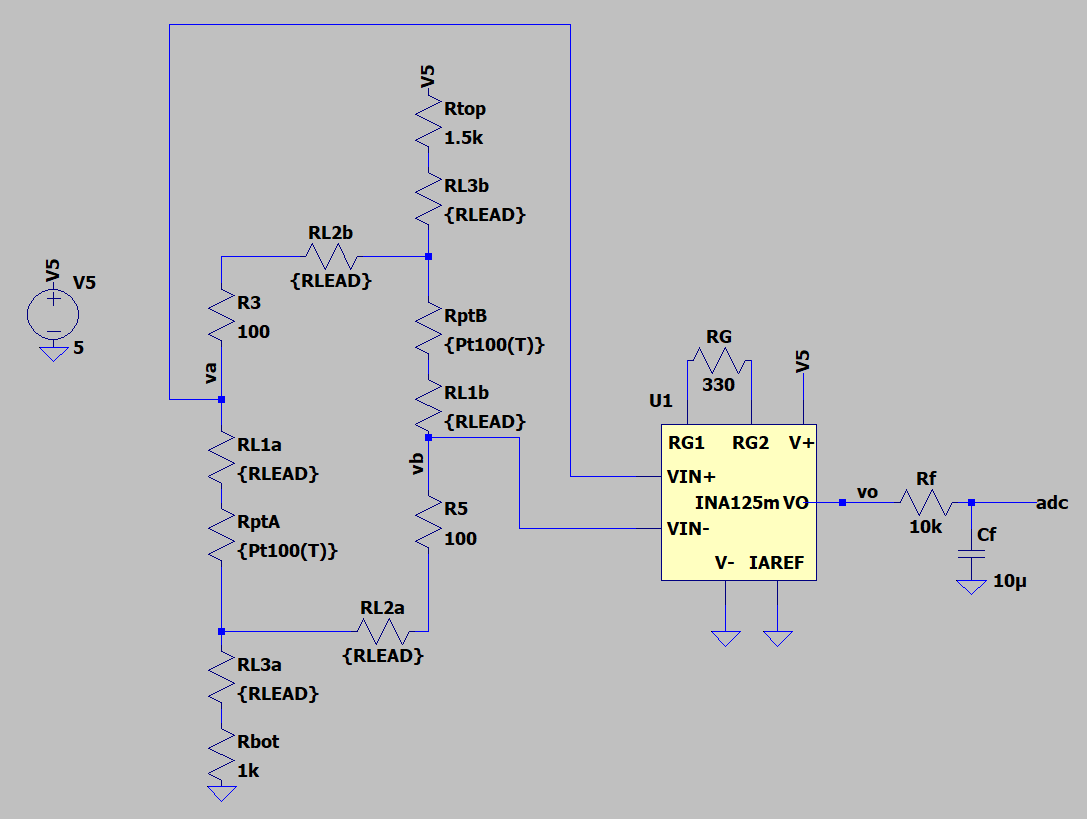
\includegraphics[width=0.85\textwidth]{lt_esq_pt100.png}
  \caption{Circuito de medição da temperatura interna simulado no LTspice, com as resistências dos fios dos Pt100 representadas explicitamente.}
  \label{fig:lt_esq_pt100}
\end{figure}

\begin{figure}[H]
  \centering
  \begin{subfigure}{\textwidth}
    \centering
    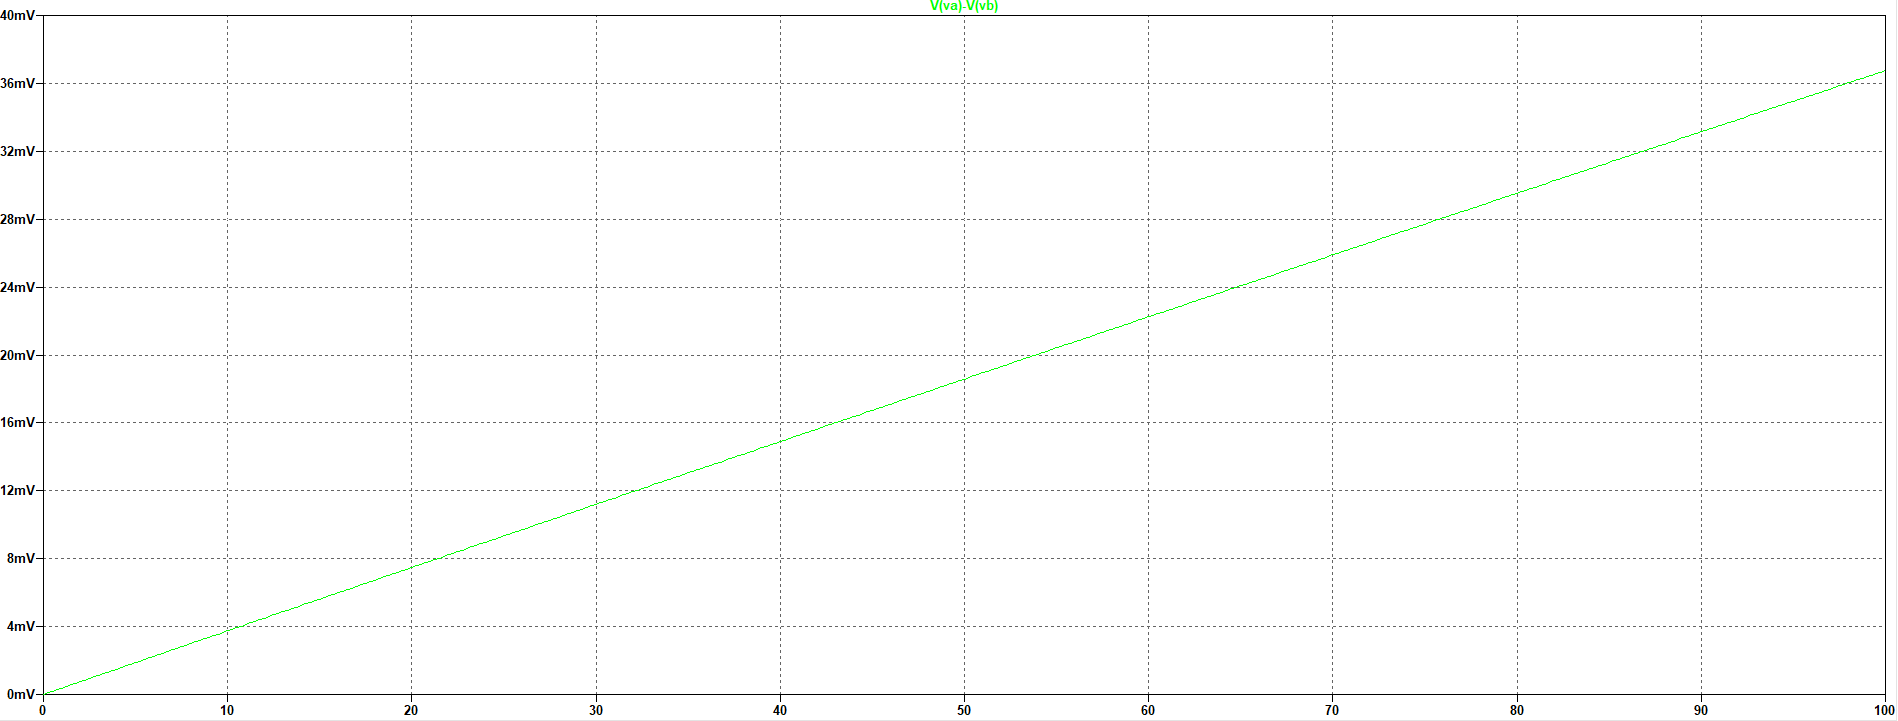
\includegraphics[width=\textwidth]{lt_vab_pt100.png}
    \caption{Saída da ponte de Wheatstone, $V_{ab} = V_a - V_b$.}
  \end{subfigure}
  \vspace{0.3cm}
  \begin{subfigure}{\textwidth}
    \centering
    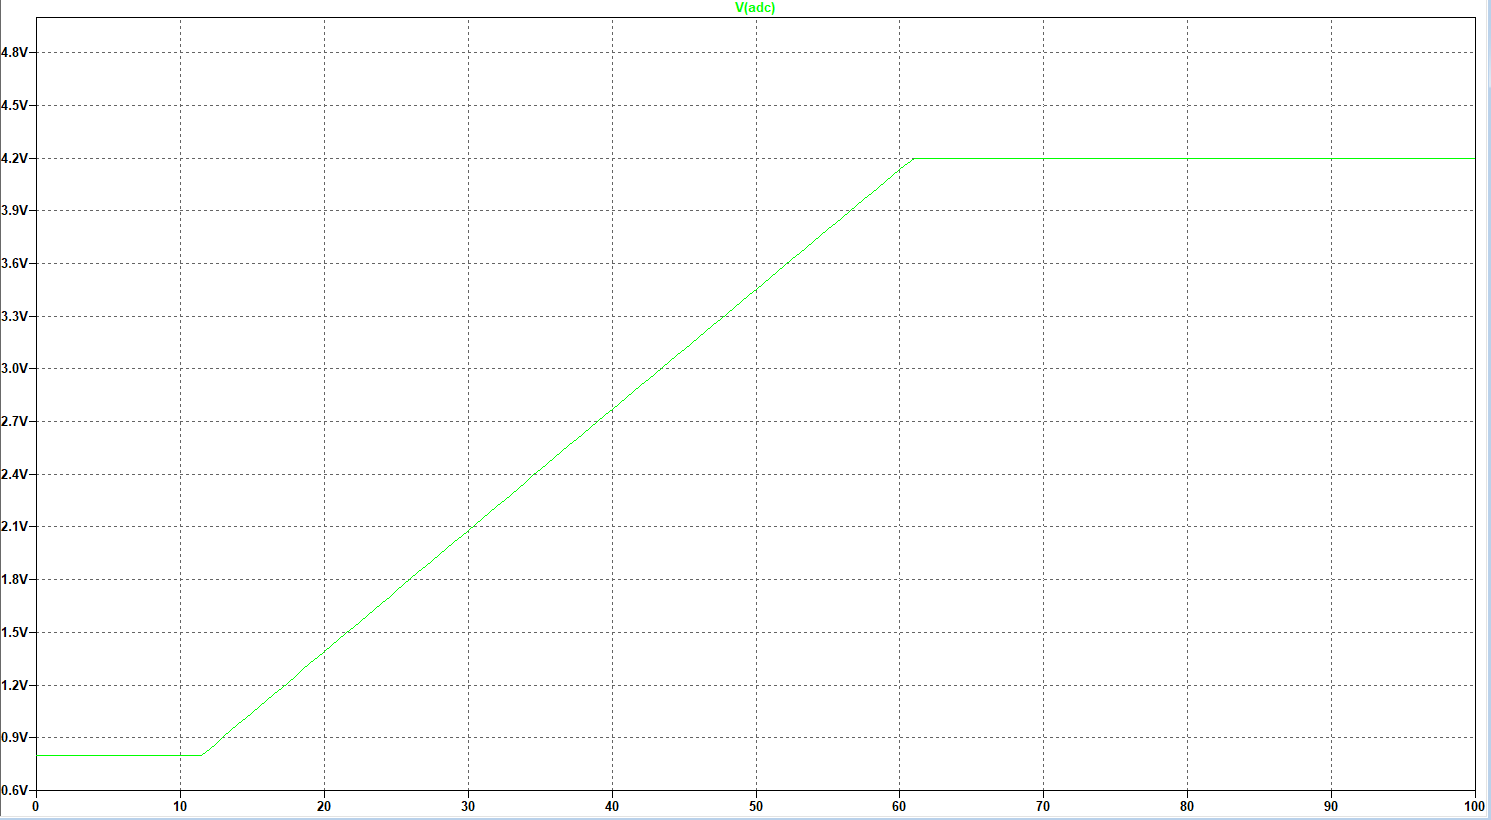
\includegraphics[width=\textwidth]{lt_vadc_pt100.png}
    \caption{Saída do INA125P após o filtro (entrada A0 do Arduino).}
  \end{subfigure}
  \caption{Resultados da simulação da medição interna. O eixo horizontal corresponde à temperatura dos Pt100, em \ensuremath{^\circ}C.}
  \label{fig:lt_sim_pt100}
\end{figure}

\begin{table}[H]
\centering
\small
\renewcommand{\arraystretch}{1.2}
\caption{Resultados simulados da medição interna.}
\label{tab:sim_pt100}
\begin{tabular}{cccc}
\toprule
\textbf{T (\ensuremath{^\circ}C)} & \textbf{$V_{ab}$ (mV)} & \textbf{$V_{out}$ (V)} & \textbf{Contagens do A/D} \\
\midrule
15 & 5,62  & 1,044 & 214 \\
20 & 7,48  & 1,390 & 284 \\
25 & 9,34  & 1,736 & 355 \\
30 & 11,20 & 2,081 & 426 \\
40 & 14,90 & 2,768 & 566 \\
50 & 18,58 & 3,452 & 706 \\
60 & 22,25 & 4,134 & 846 \\
\bottomrule
\end{tabular}
\end{table}

Os principais resultados são:
\begin{itemize}
  \item sensibilidade de 68,7\,mV/\ensuremath{^\circ}C e resolução de 0,071\,\ensuremath{^\circ}C por LSB;
  \item faixa útil de 12\,\ensuremath{^\circ}C a 61\,\ensuremath{^\circ}C, limitada pela excursão de saída do INA125P;
  \item erro de não linearidade de no máximo 0,11\,\ensuremath{^\circ}C entre 15 e 60\,\ensuremath{^\circ}C, o que justifica a conversão linear;
  \item com resistência exagerada de 1\,$\Omega$ em cada fio, o erro foi de apenas $-$0,02\,\ensuremath{^\circ}C a 50\,\ensuremath{^\circ}C com a ligação a 3 fios, contra +5,2\,\ensuremath{^\circ}C em uma ligação a 2 fios equivalente.
\end{itemize}

\subsection{Acionamento}

O circuito da Figura~\ref{fig:lt_esq_acion} foi simulado com PWM de 490\,Hz e razão cíclica de 50\,\%. A indutância parasita dos resistores de aquecimento foi representada por $L_{heat}$ = 2\,$\mu$H. O terra do Arduino (\textit{gard}) é isolado do terra da fonte pelo optoacoplador; o resistor $R_{gnd}$ existe apenas para que o simulador tenha uma referência comum. As formas de onda são apresentadas na Figura~\ref{fig:lt_formas_acion}.

\begin{figure}[H]
  \centering
  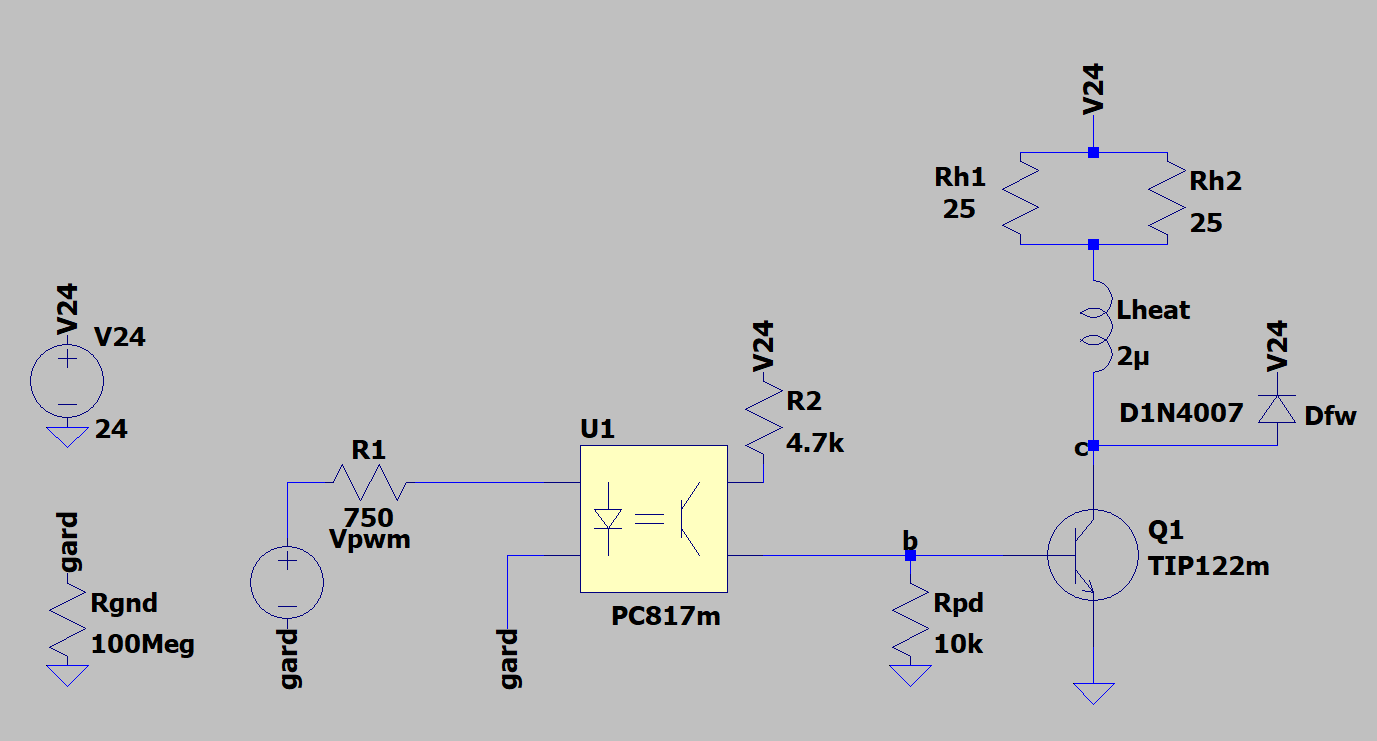
\includegraphics[width=0.9\textwidth]{lt_esq_acion.png}
  \caption{Circuito de acionamento simulado no LTspice: optoacoplador PC817, transistor Darlington TIP122 e placa com três resistores de 15\,$\Omega$ em paralelo, alimentada em 12\,V.}
  \label{fig:lt_esq_acion}
\end{figure}

\begin{figure}[H]
  \centering
  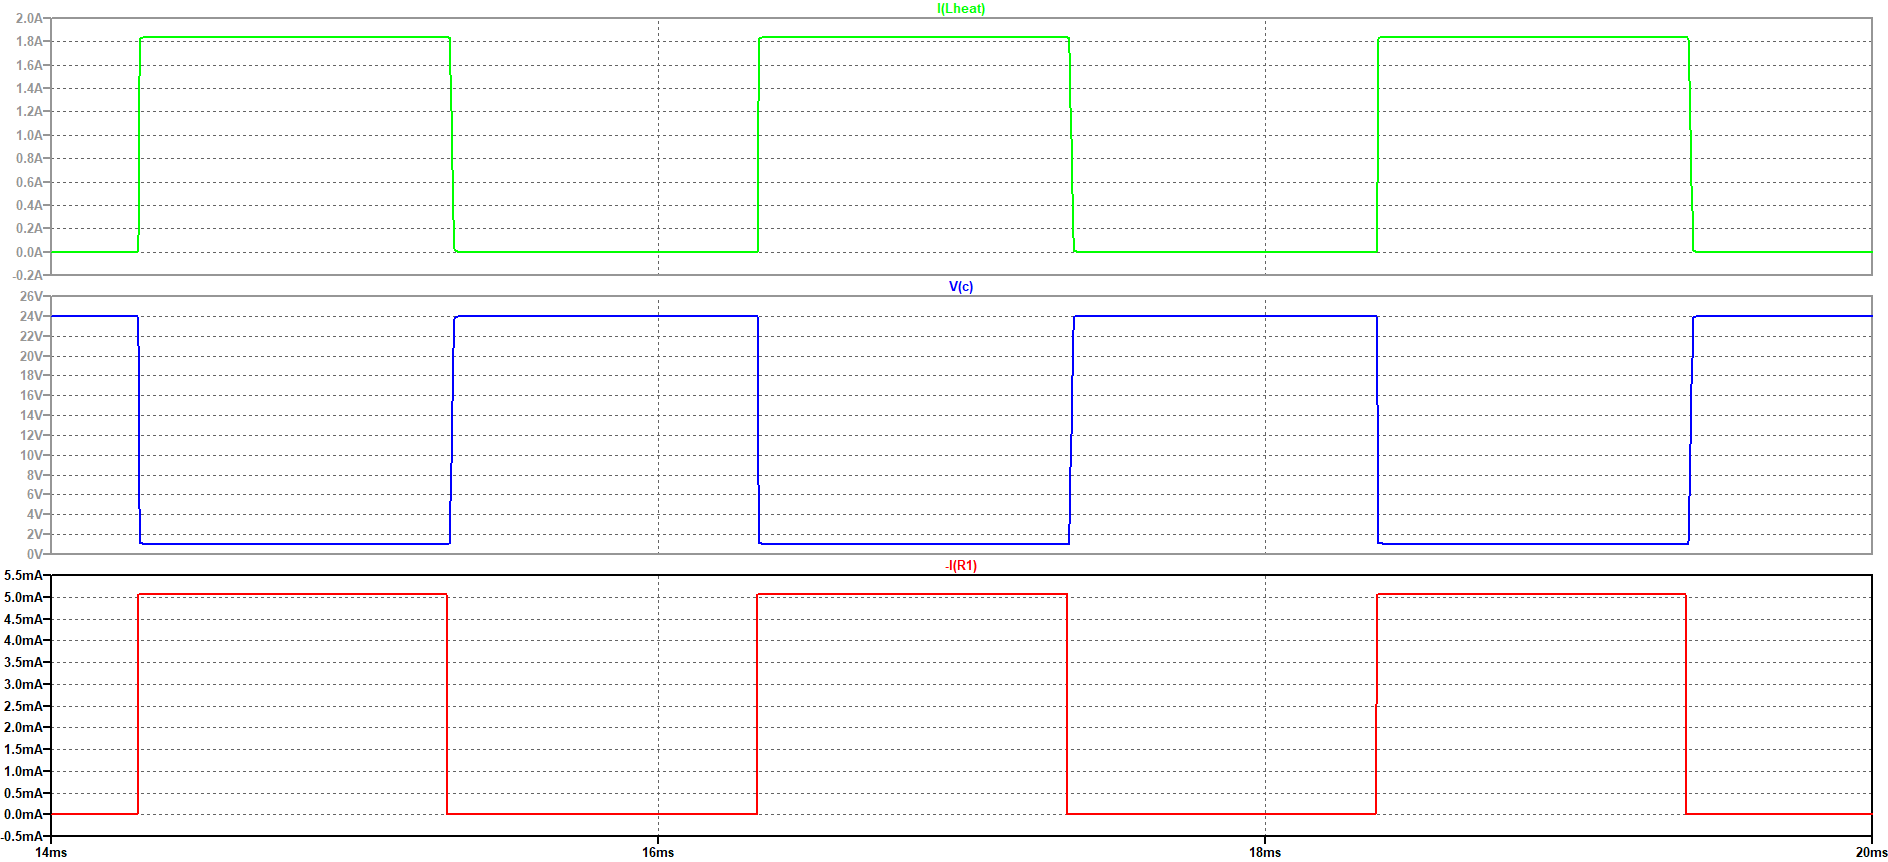
\includegraphics[width=\textwidth]{lt_formas_acion.png}
  \caption{Formas de onda simuladas do acionamento (PWM de 490\,Hz, D = 50\,\%): corrente no aquecedor, tensão no coletor do TIP122 e corrente no LED do PC817.}
  \label{fig:lt_formas_acion}
\end{figure}

Os principais resultados são:
\begin{itemize}
  \item corrente de 2,17\,A no aquecedor durante a condução, com o TIP122 saturado ($V_{CE} \approx 1{,}13$\,V);
  \item corrente de 5,6\,mA no LED do PC817 e cerca de 2,7\,mA na base do TIP122, acima do mínimo de 2,2\,mA necessário para a saturação;
  \item potência média de 12,2\,W no aquecedor e de 1,3\,W no TIP122 com razão cíclica de 50\,\%, ou seja, cerca de 24\,W e 2,6\,W em 100\,\%;
  \item tensão máxima de 12,1\,V no coletor durante o desligamento, limitada pelo diodo de roda livre.
\end{itemize}
